We evaluate five knowledge injection strategies on a benchmark of 50 yes/no questions requiring knowledge of counterintuitive scientific facts. Each method represents a distinct approach to addressing LLM knowledge gaps.

\subsection{Zero-Shot (Baseline)}
The zero-shot baseline uses a simple prompt: ``Answer yes/no questions with ONLY yes or no.'' We use temperature $T=0.1$ to minimize randomness. No knowledge injection or reasoning steps are applied. This tests the model's innate knowledge without any augmentation.

\subsection{Chain-of-Thought (CoT)}
The CoT prompt instructs: ``Think step by step, then answer YES or NO.'' We use temperature $T=0.3$ to allow some diversity while maintaining consistency. No knowledge is injected. This tests whether reasoning-step guidance alone helps on knowledge-sensitive questions.

\subsection{Self-Consistency Without KB (SC-only)}
We sample 7 independent reasoning paths at temperature $T=0.5$ with the CoT prompt. The final answer is determined by majority vote. This tests whether reasoning diversity alone can overcome knowledge gaps. The assumption is that if the model knows the answer, multiple reasoning paths should converge on it.

\subsection{Simple RAG (Naive Knowledge Injection)}
Knowledge base facts are placed directly in the system prompt. We use a single forward pass at $T=0.3$. This tests whether naive knowledge injection---without any structural guidance on how to use the facts---helps. The knowledge base contains 19 curated scientific facts covering physics, chemistry, biology, and common misconceptions.

\subsection{KB+SC with Step 1/Step 2 (Our Method)}
Our proposed method combines three components: (1) knowledge base in system prompt, (2) 7-path self-consistency voting, and (3) a structured Step 1/Step 2 prompt that forces explicit knowledge scanning:

\begin{algorithm}[h]
\caption{KB+SC+Step1/2 Method}
\begin{algorithmic}[1]
\REQUIRE Question $q$, Knowledge Base $KB$, Number of SC paths $n=7$
\ENSURE Final answer
\FOR{$i = 1$ to $n$}
    \STATE Sample reasoning path at $T=0.5$
    \STATE \textbf{Step 1:} ``Does any fact in the knowledge base directly relate to this question? If yes, state it.''
    \STATE \textbf{Step 2:} ``Based on the knowledge base, answer YES or NO.''
    \STATE Record answer $a_i$
\ENDFOR
\STATE \textbf{Return} Majority vote of $\{a_1, ..., a_n\}$
\end{algorithmic}
\end{algorithm}

This method forces the model to explicitly scan for relevant knowledge base facts before answering, rather than passively receiving context. The Step 1/Step 2 structure ensures that relevant knowledge is identified and applied, preventing both fact ignoring and fact misapplication.

\subsection{Knowledge Base Construction}
Our knowledge base contains 19 curated scientific facts covering areas where LLMs commonly fail:

\begin{itemize}
\item \textbf{Physics:} Diamonds can burn (pure carbon), hot water can freeze faster than cold (Mpemba effect), sound cannot travel in vacuum
\item \textbf{Chemistry:} Gold is chemically inert, water expands when freezing, noble gases are reactive under certain conditions
\item \textbf{Biology:} Octopuses have three hearts, bananas are radioactive, human body contains enough carbon to make ~9000 pencils
\item \textbf{Common misconceptions:} Lightning can strike the same place twice, bulls are not angered by red color, goldfish have longer memories than commonly believed
\end{itemize}

\subsection{Pipeline Diagram}
Figure~\ref{fig:pipeline} shows the overall system architecture comparing naive RAG versus our structured KB+SC+Step1/2 approach.

\begin{figure}[t]
\centering
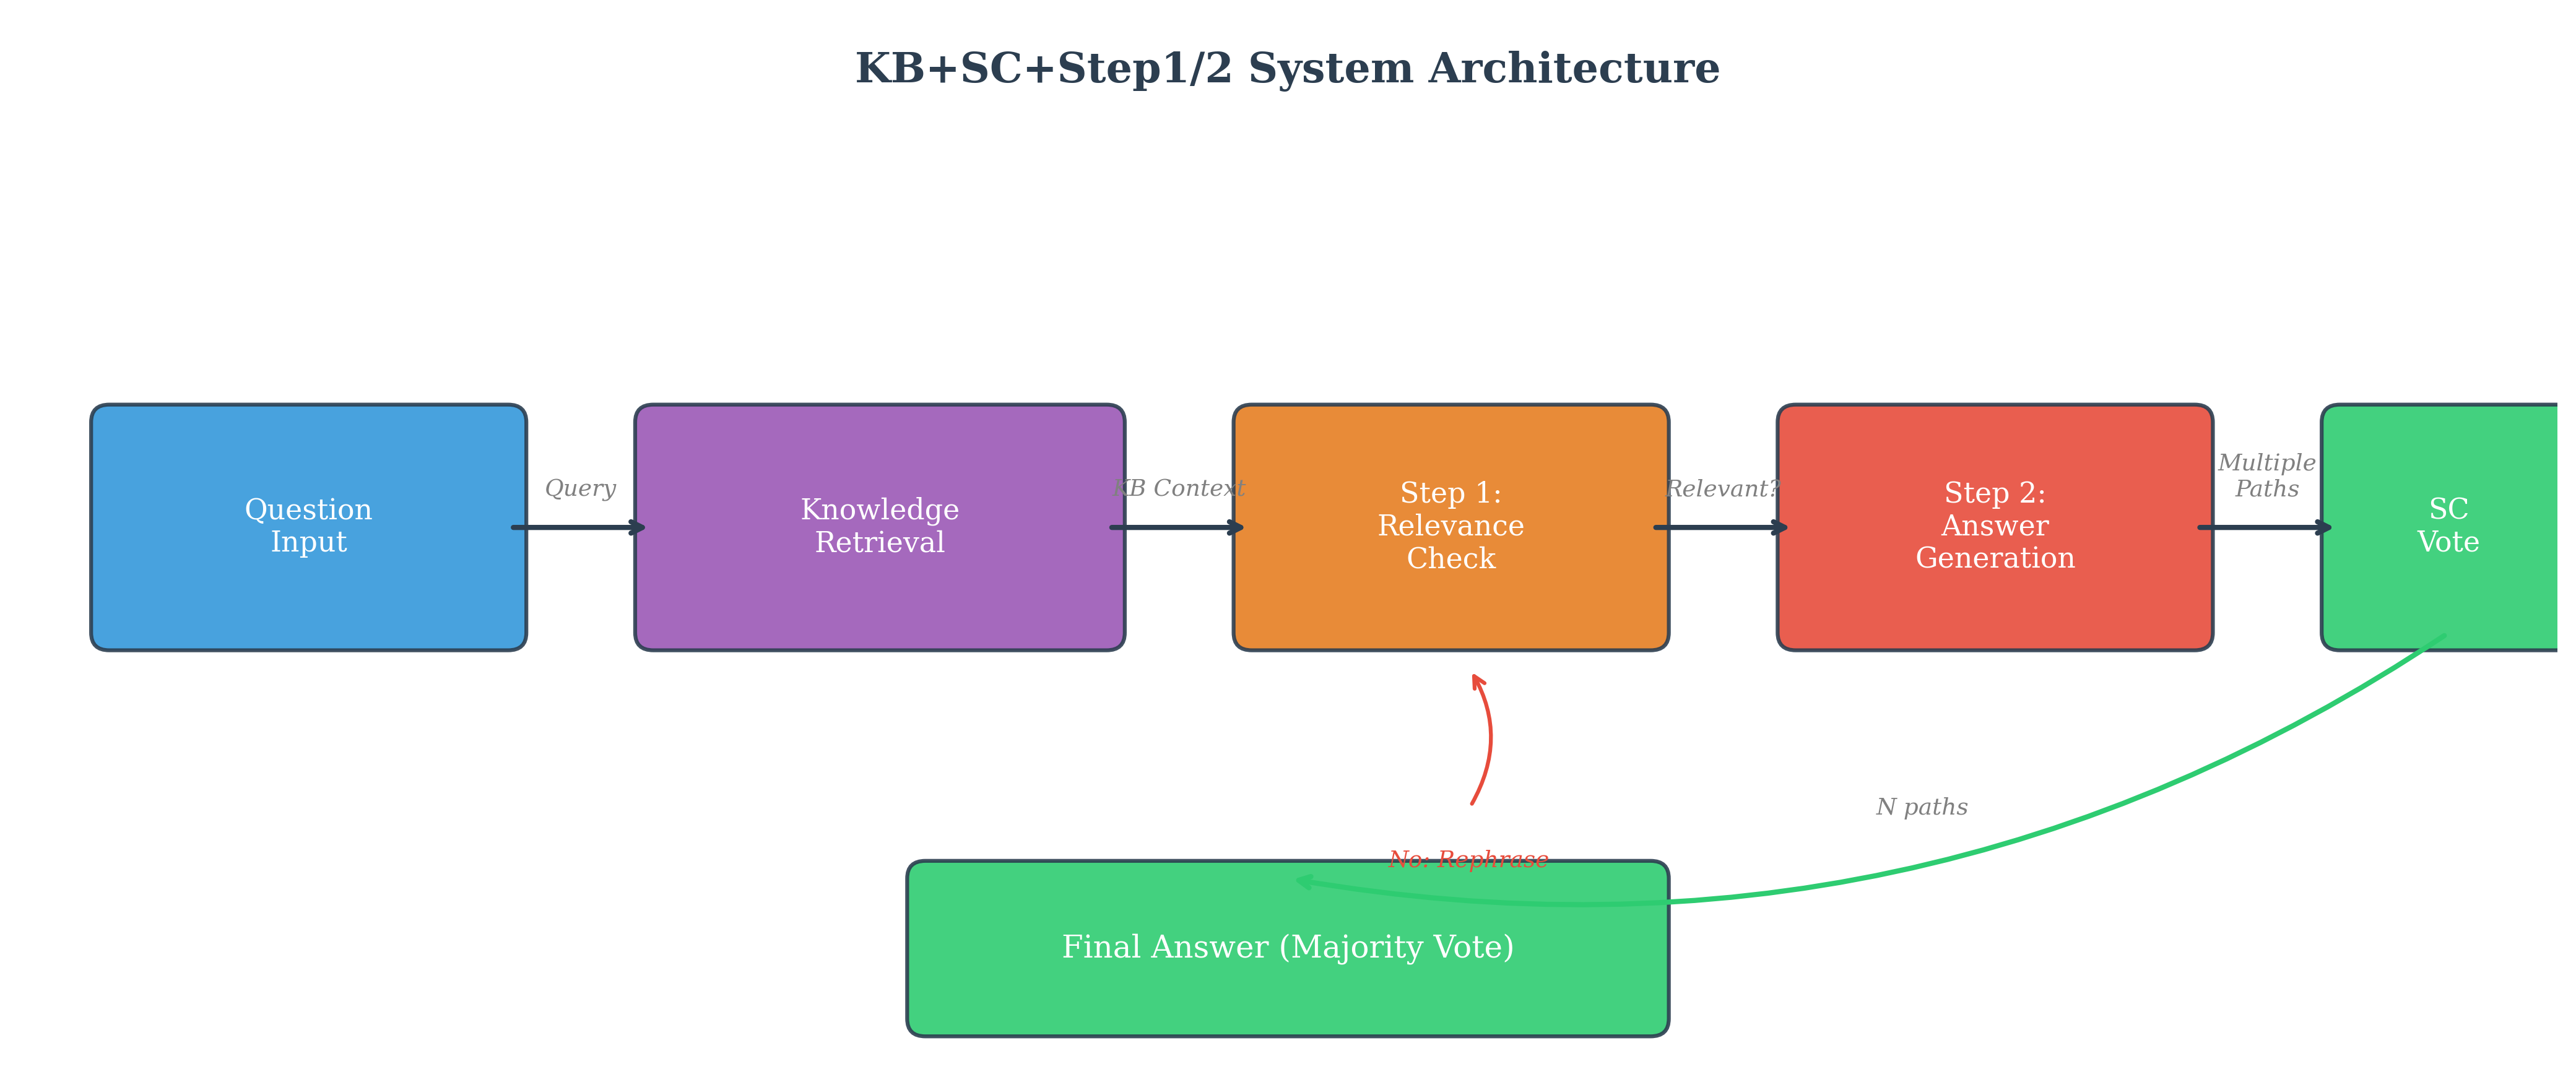
\includegraphics[width=0.95\columnwidth]{figures/fig5_architecture.png}
\caption{System architecture comparison: Naive RAG places knowledge directly in context (left), while KB+SC+Step1/2 forces explicit knowledge scanning through structured prompting (right).}
\label{fig:pipeline}
\end{figure}
